A pesquisa e o desenvolvimento (P\&D) tem como propósito fomentar o avanço
tecnológico e novas maneiras de desenvolver tipos específicos de conhecimento
no país. O desenvolvimento do robô EMMA, no âmbito P\&D é um exemplo de como a
parceria entre agências do governo e uni- versidades federais podem colaborar
para a capacitação tecnológica e o desenvolvimento de novas tecnologias.
Especificamente na área de robó\-tica, o projeto EMMA mostra como a otimização e
automação de diversos processos pode contribuir na indústria
energética. Em termos acadêmicos, esta linha de projetos possibilitou a
realização de duas
dissertações de mestrado, uma no Programa de Engenharia Elétrica (PEE),
Universidade Federal do Rio de Janeiro (UFRJ), e outra no Departamento
de Artes e Design (PPGDesign), assim como uma graduação em engenharia
Mecânica na Universidade do Vale do Rio dos Sinos

Seguem as declarações e histórico de comprovação de mestrado e graduação.

%, abordando os seguintes
% tópic%TODO Julia e Estevao - Propostas

%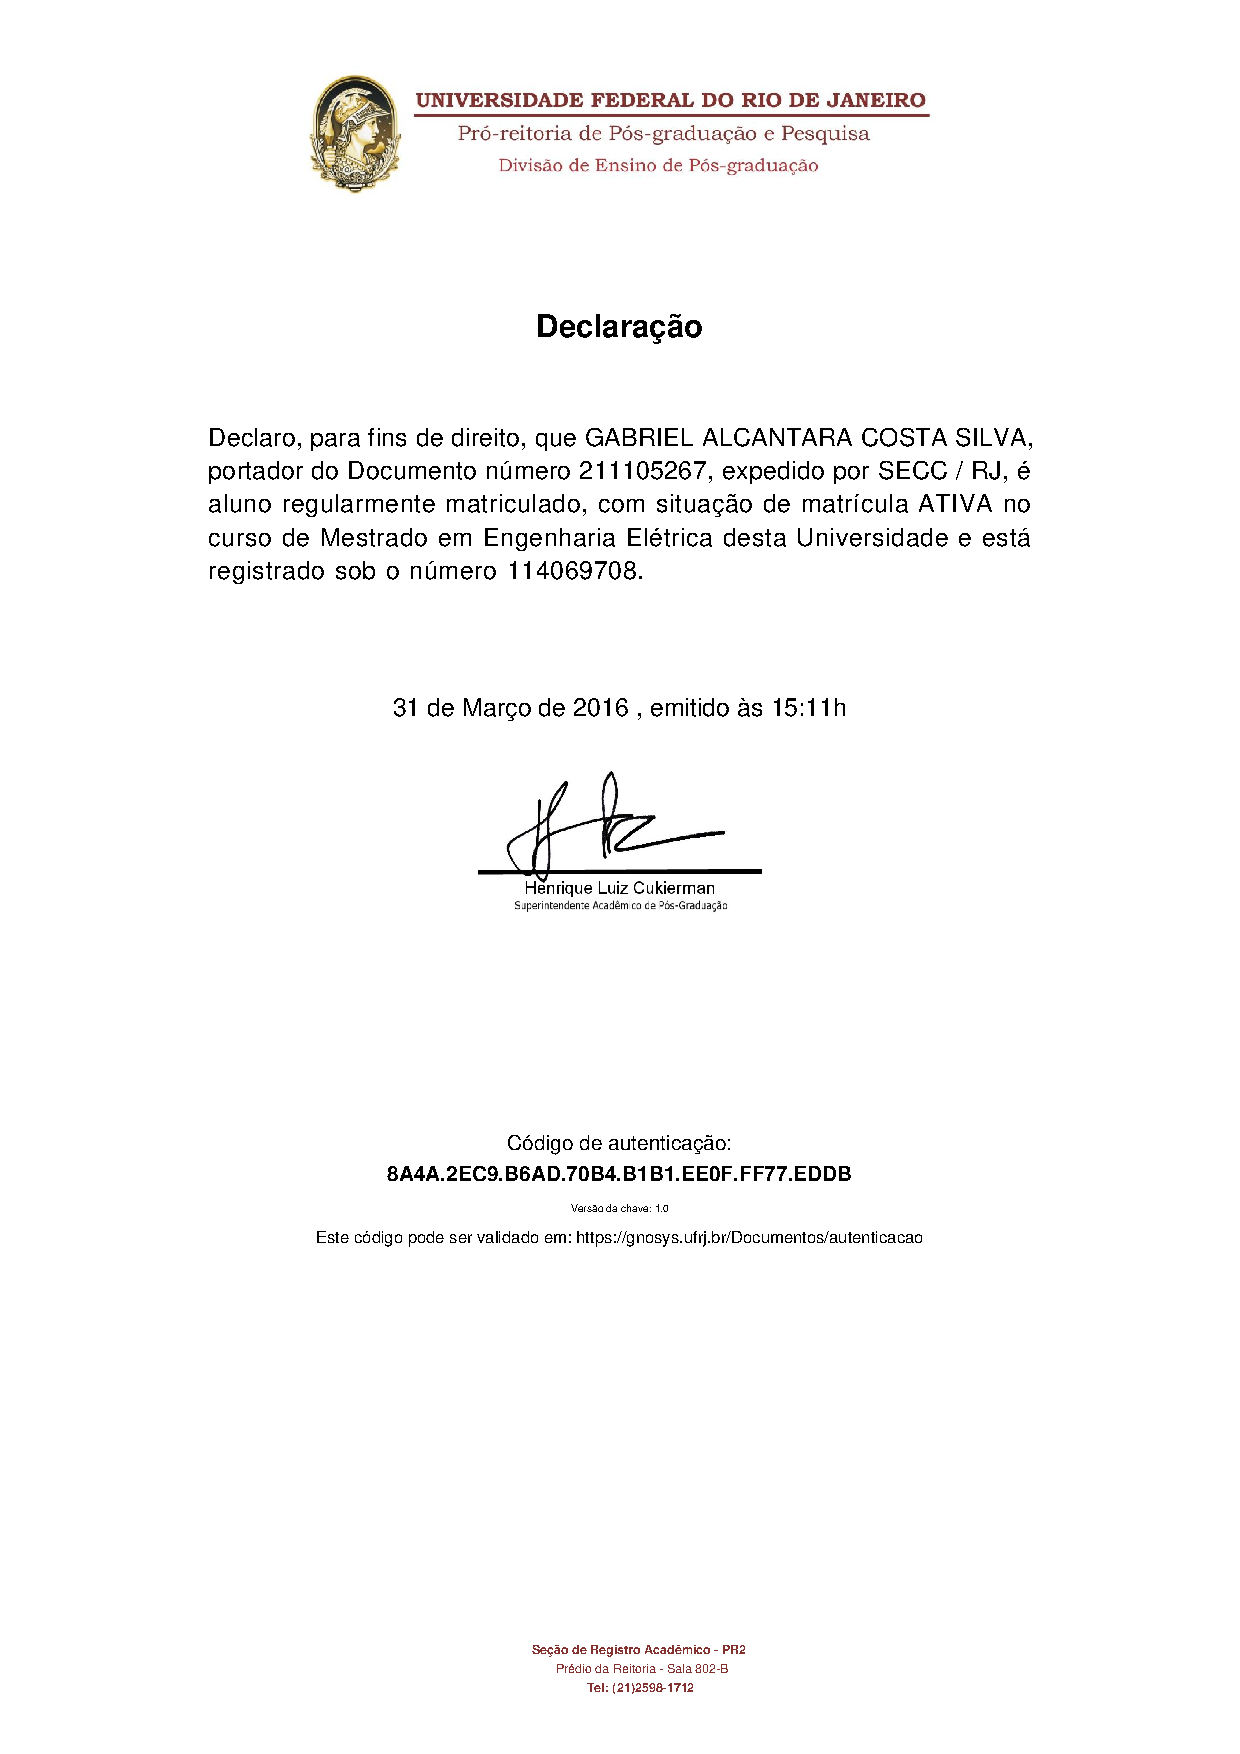
\includepdf{pdfs/mestrado_gabriel}
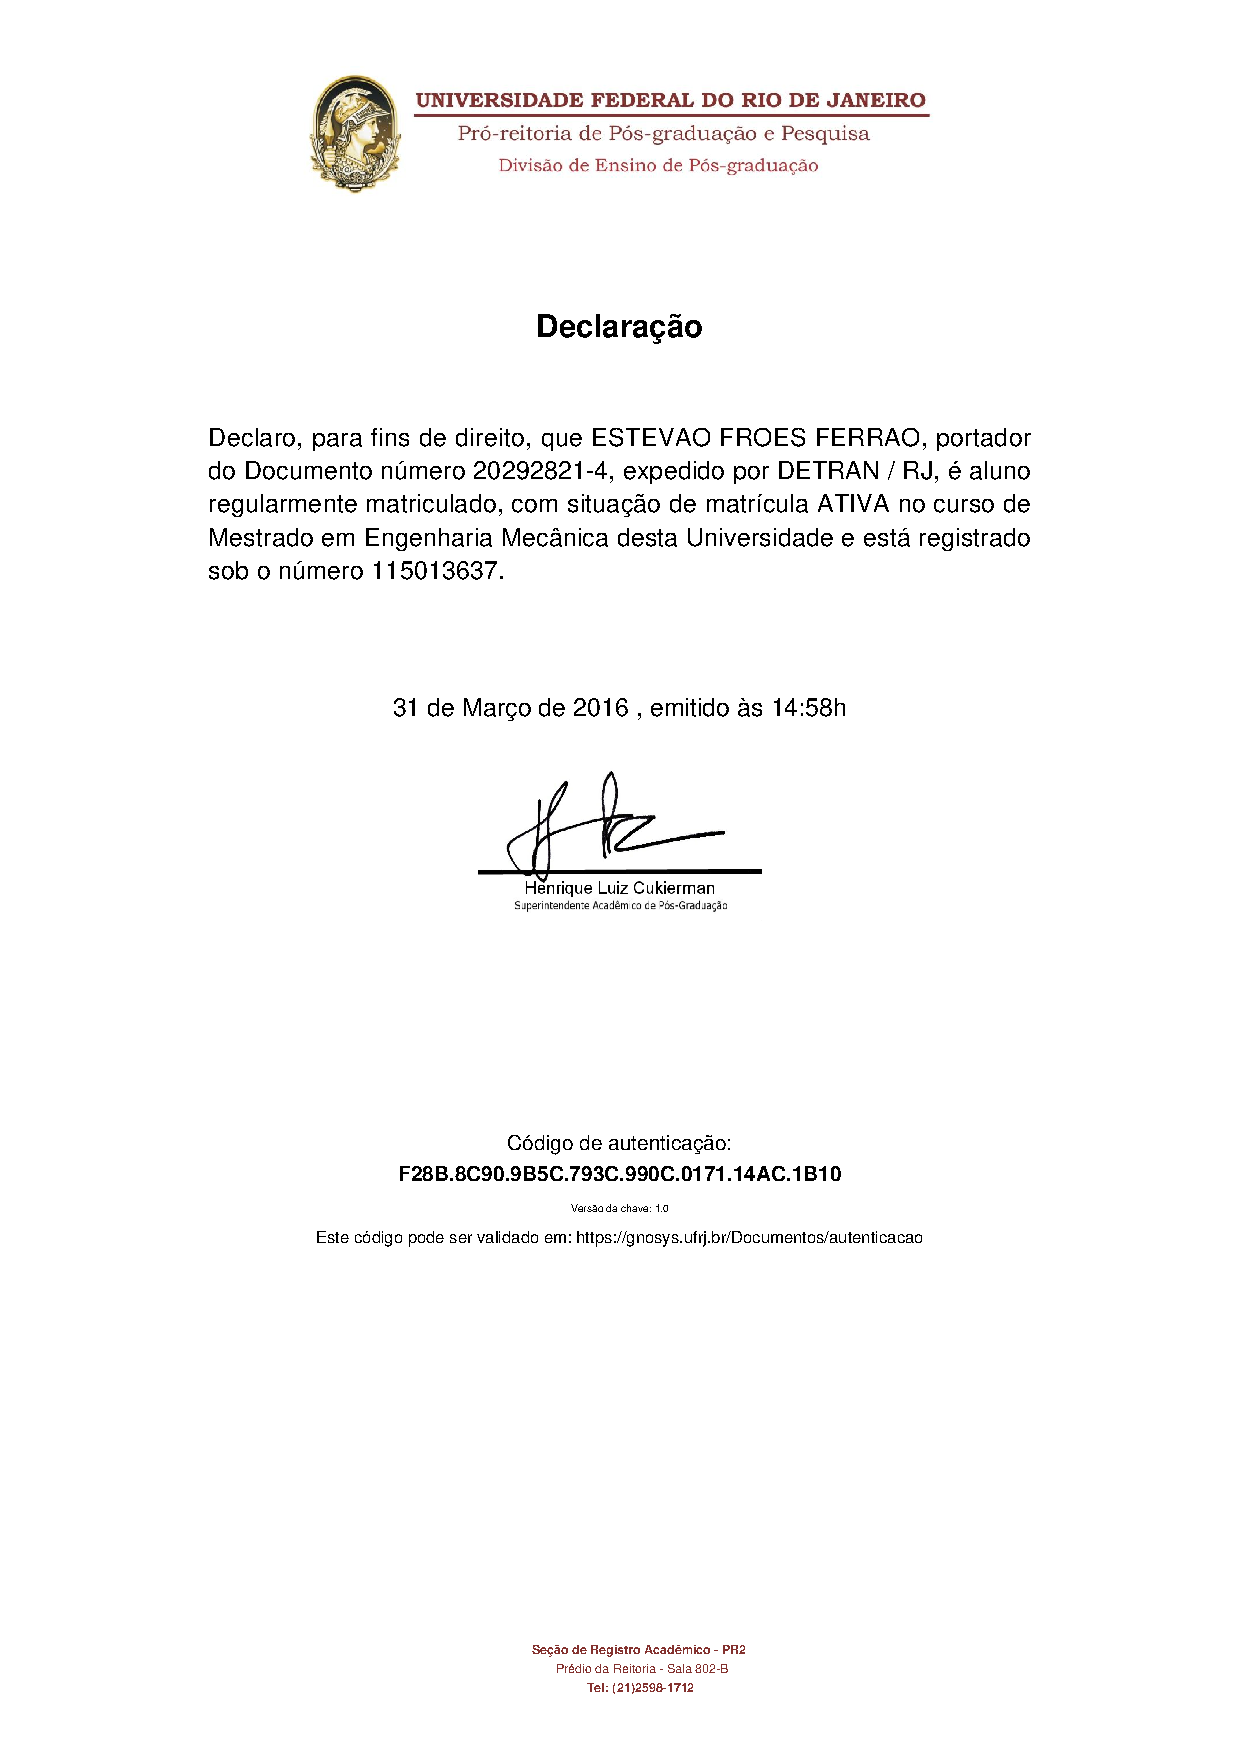
\includepdf{pdfs/mestrado_estevao}
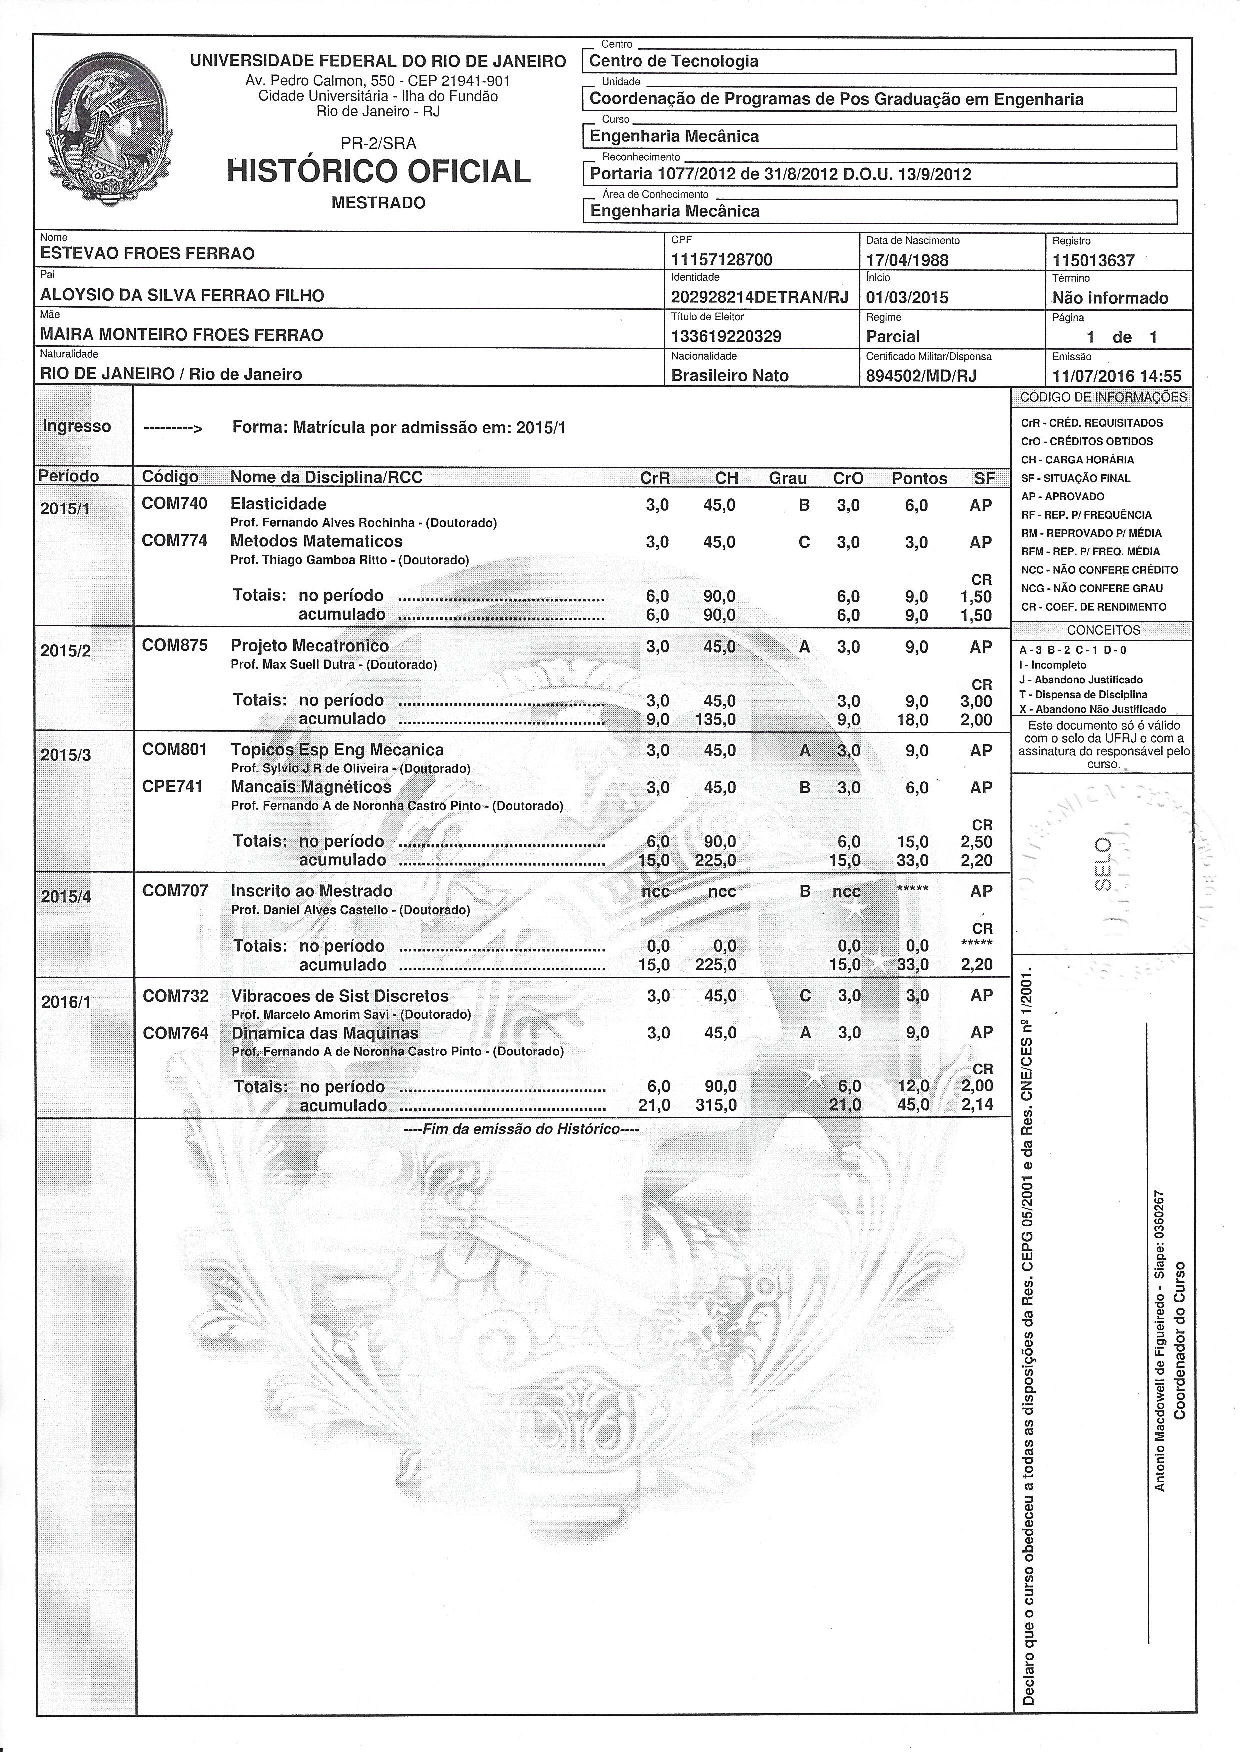
\includepdf[pages=1-]{pdfs/historico_estevao}
%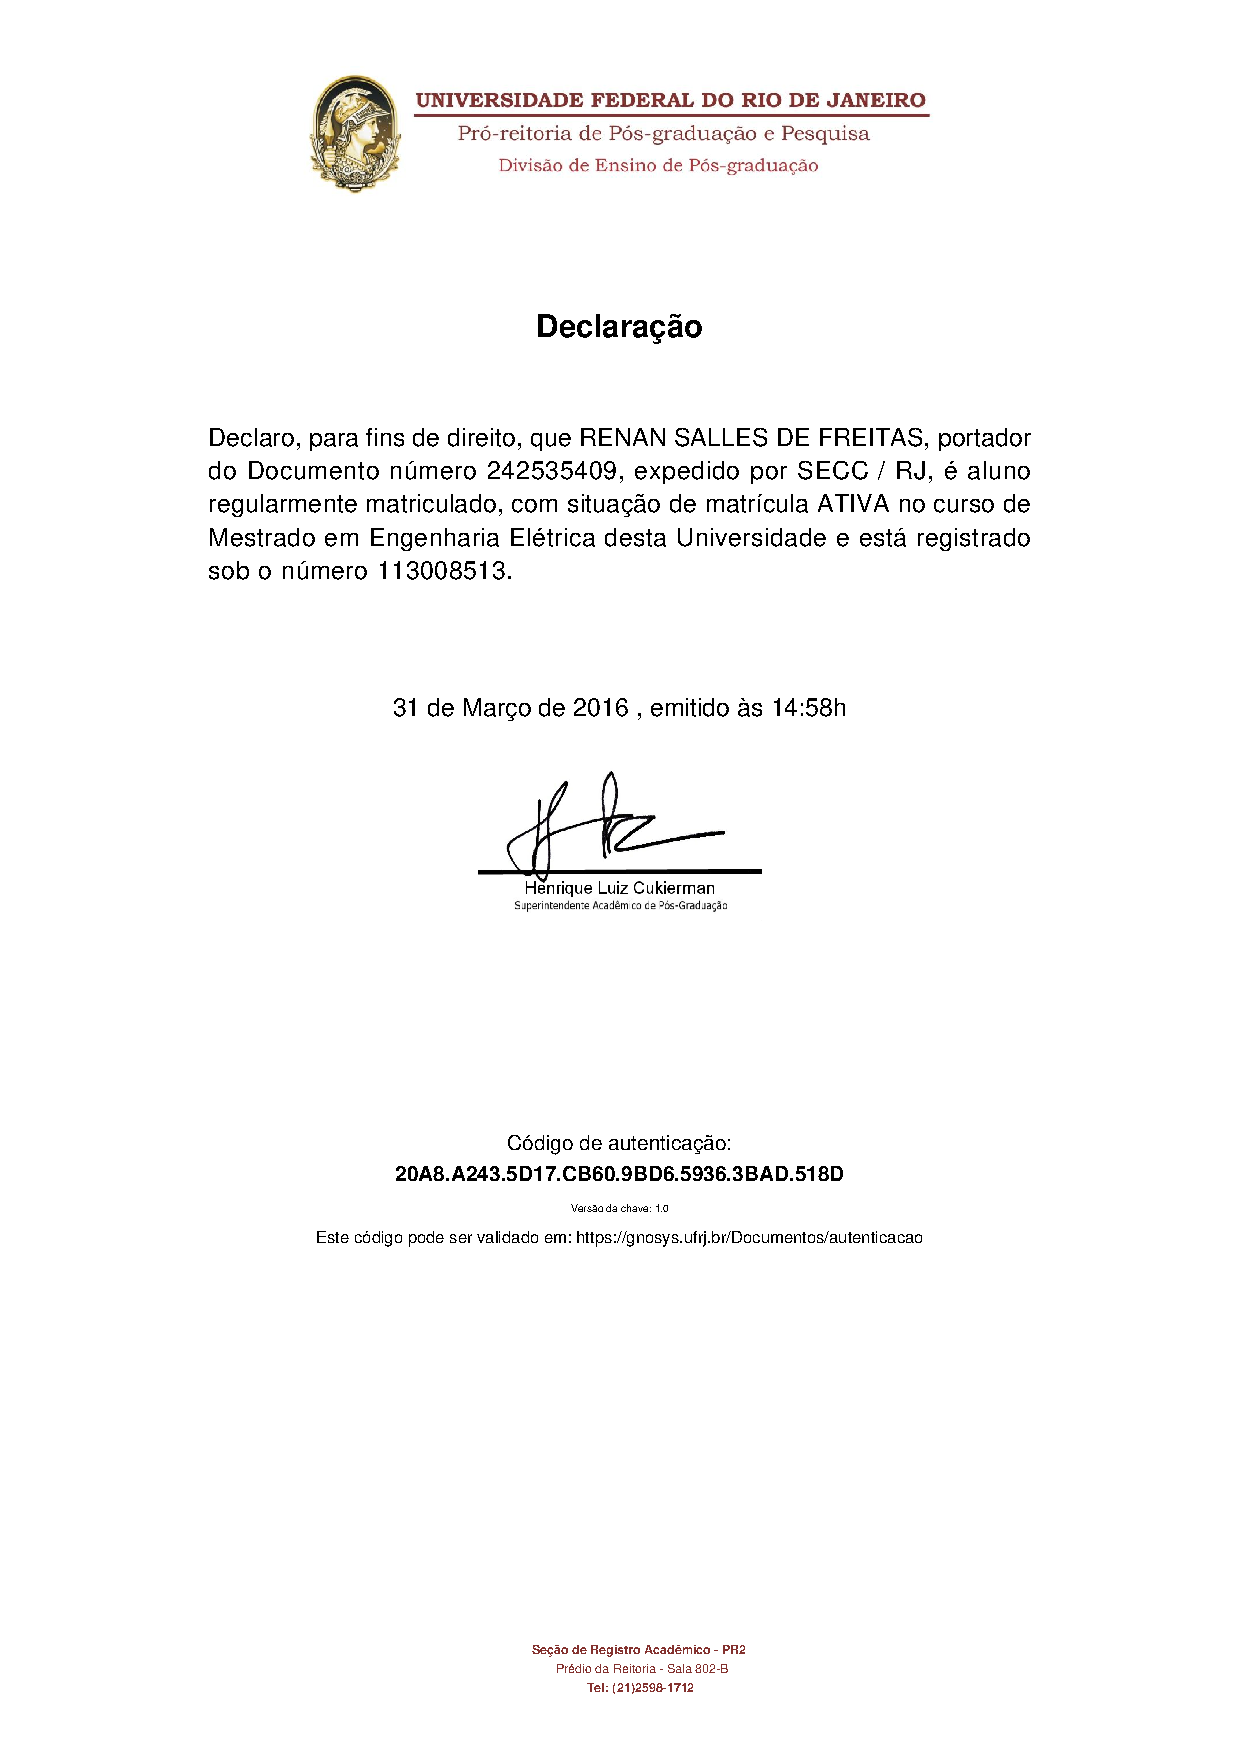
\includepdf{pdfs/mestrado_renan}
%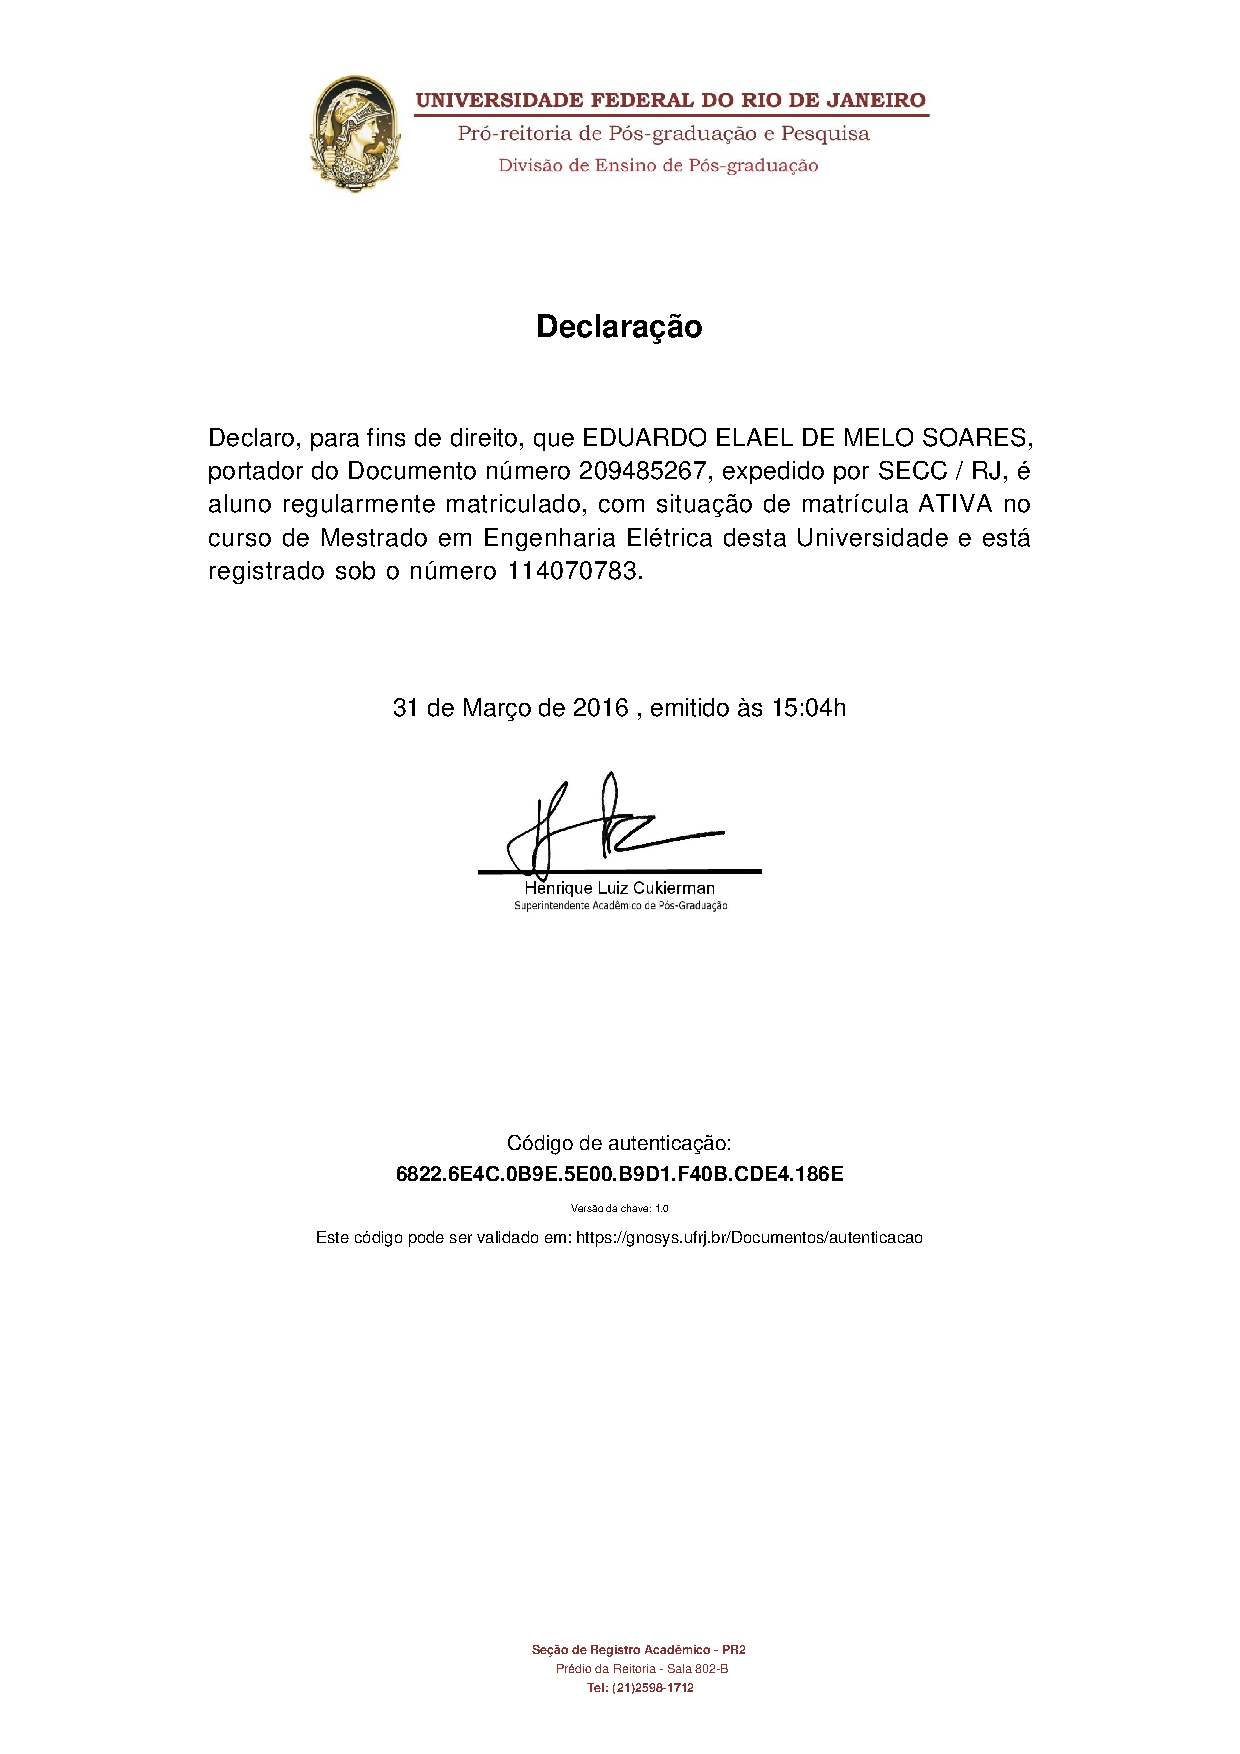
\includepdf{pdfs/mestrado_elael}
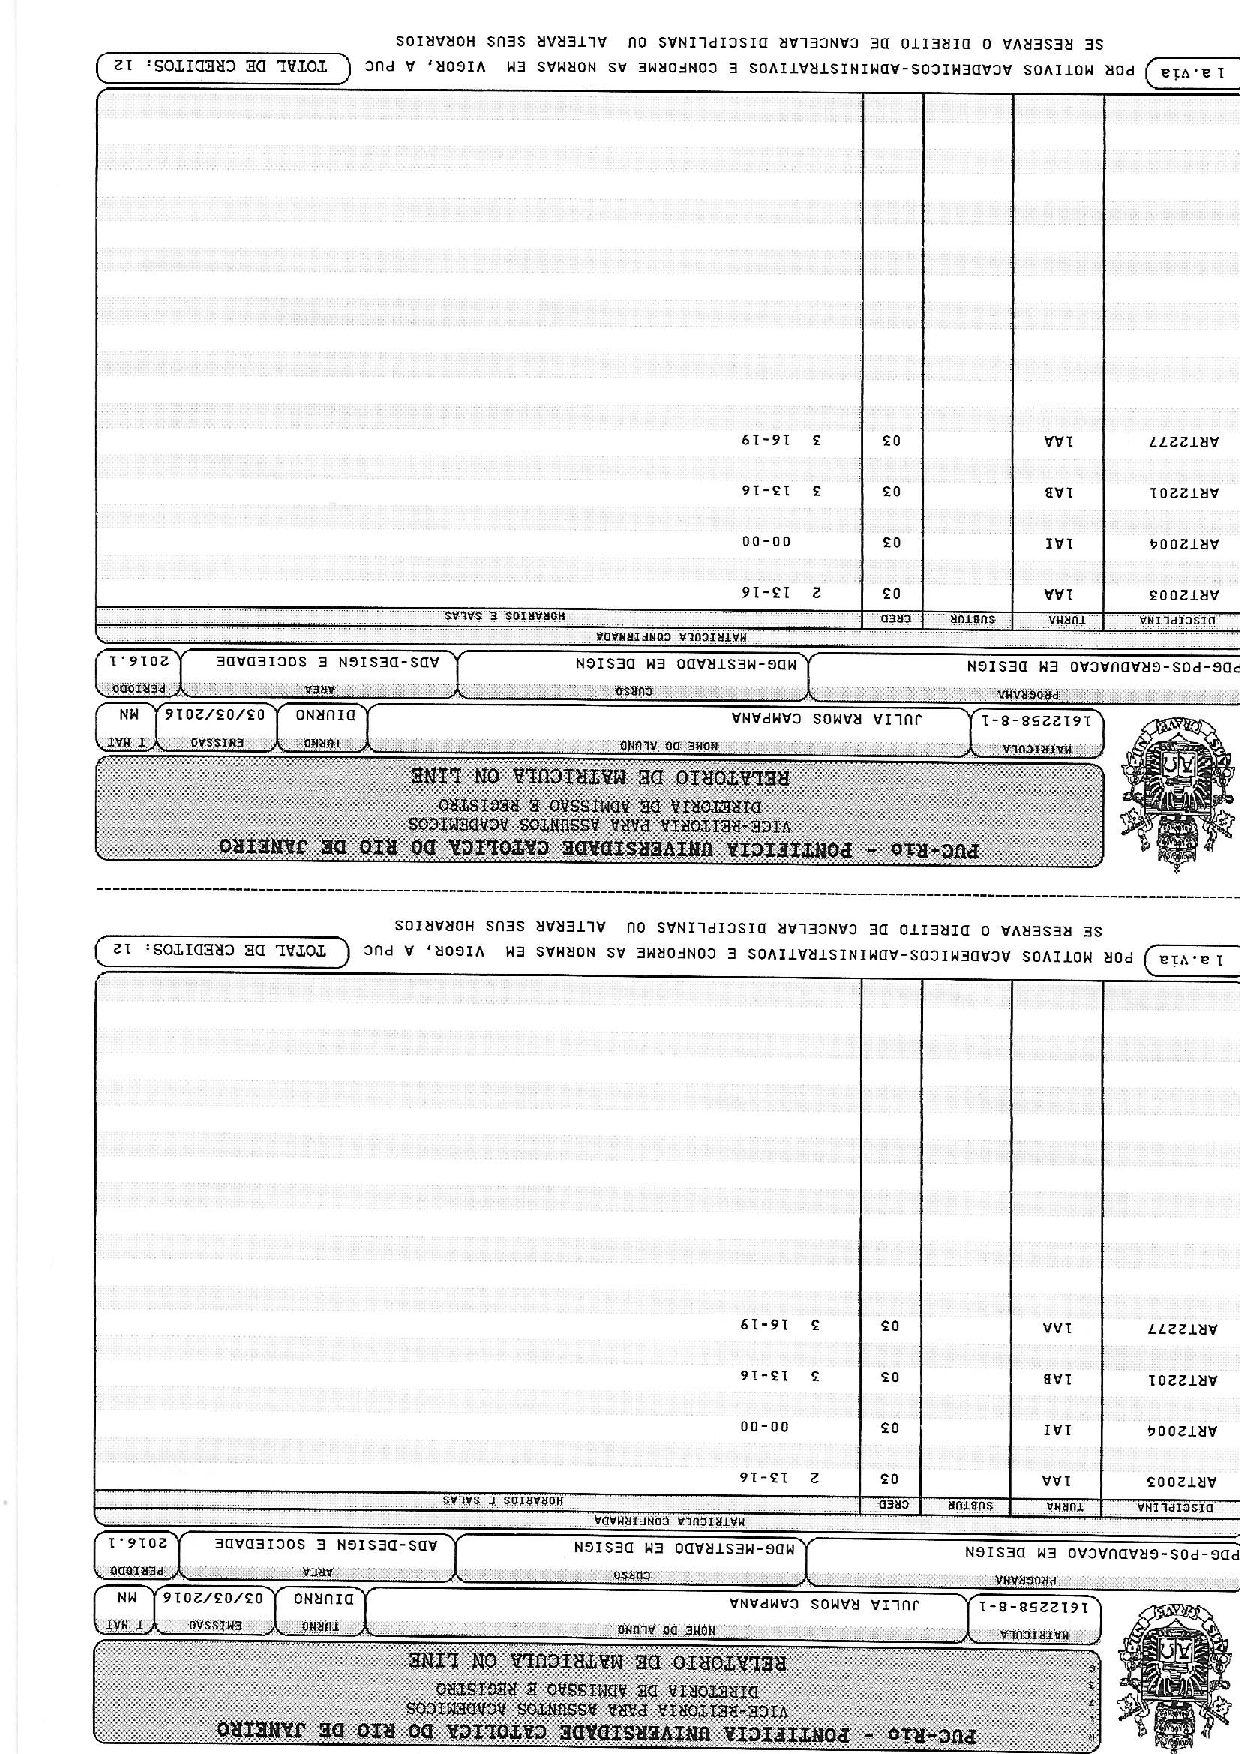
\includepdf[angle=180]{pdfs/mestrado_julia}
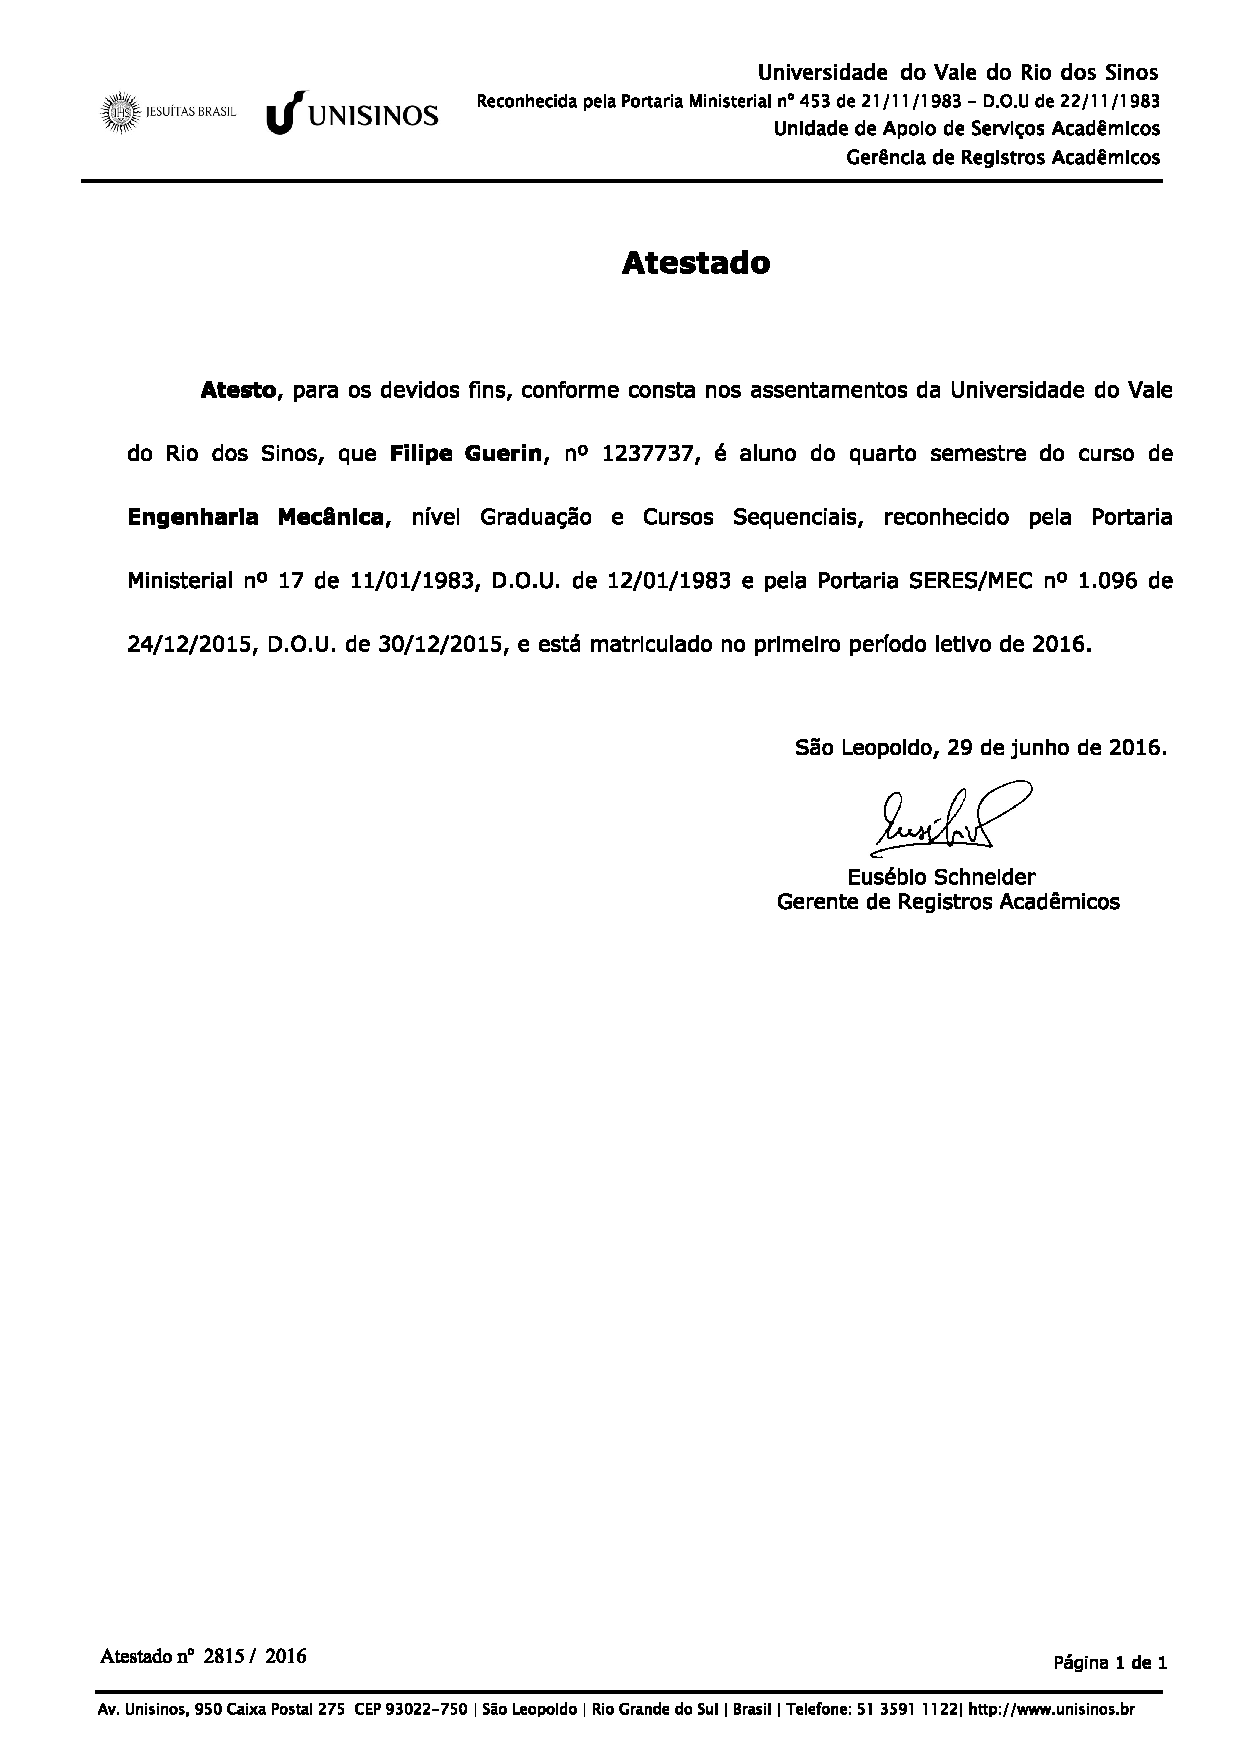
\includepdf{pdfs/graduacao_guerin}
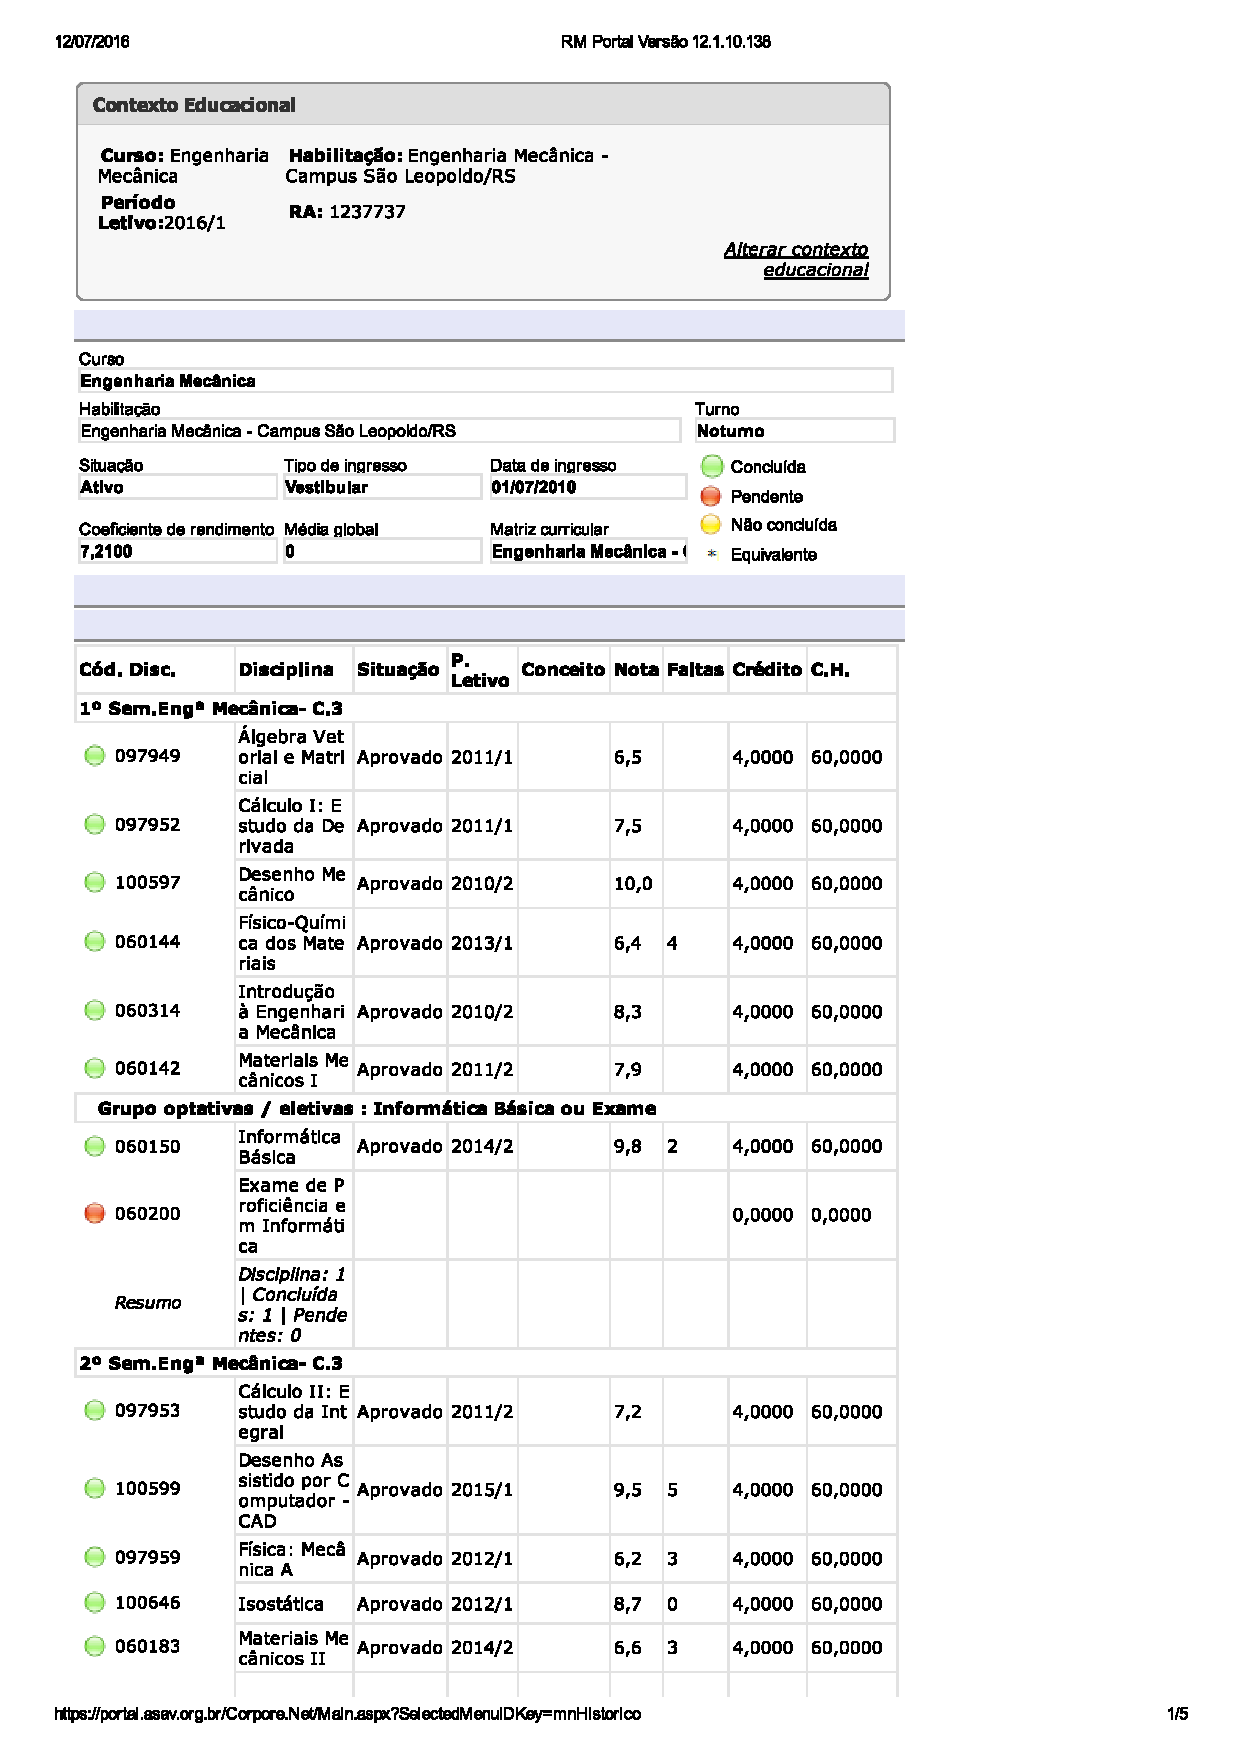
\includepdf[pages=1-]{pdfs/historico_guerin}

